\documentclass[12pt, titlepage]{article}

\usepackage{fullpage}
\usepackage[round]{natbib}
\usepackage{multirow}
\usepackage{booktabs}
\usepackage{tabularx}
\usepackage{graphicx}
\usepackage{float}
\usepackage[normalem]{ulem}
\usepackage[colorlinks]{hyperref}
\hypersetup{
    colorlinks,
    citecolor=black,
    filecolor=black,
    linkcolor=red,
    urlcolor=blue
}
\usepackage[round]{natbib}

\newcounter{acnum}
\newcommand{\actheacnum}{AC\theacnum}
\newcommand{\acref}[1]{AC\ref{#1}}

\newcounter{ucnum}
\newcommand{\uctheucnum}{UC\theucnum}
\newcommand{\uref}[1]{UC\ref{#1}}

\newcounter{mnum}
\newcommand{\mthemnum}{M\themnum}
\newcommand{\mref}[1]{M\ref{#1}}

\title{SE 3XA3: Module Guide\\CamRuler}

\author{Team 10,
		\\ Kshitij Mehta, mehtak1
		\\ Meet Patel, patelm16
		\\ Prince Kowser, kowserm
}

\date{\today}

\begin{document}

\maketitle

\pagenumbering{roman}
\tableofcontents
\listoftables
\listoffigures


\begin{table}
\caption{\bf Revision History}
\begin{tabularx}{\textwidth}{p{3cm}p{2cm}X}
\toprule {\bf Date} & {\bf Version} & {\bf Notes}\\
\midrule
Nov.11,2017 & 1.0  & Revision 0 Complete \\
\midrule
Dec.6,2017 & 1.1r & Revision 1 Complete \\
\bottomrule
\end{tabularx}
\end{table}

\newpage

\pagenumbering{arabic}

\section{Introduction}


The CamRuler application is a re-implementation of an existing open-source Android application which enables a user to get measurements of an object through taking a picture. 
\\

\noindent This document is the Module Guide (MG) and is created after the Software Requirements Specification (SRS). The main purpose of the SRS is to specify all the functional and non-functional requirements for the project, compared to the MG which provides a modular decomposition of the system to display the modular structure of it. The MG also documents how the system meets both functional and non-functional requirements specified in the SRS. The Module Interface Specification (MIS) is created after the MG which MIS explains the semantics (state and environment variables, assumptions, and access routines) and syntax of exported functions (input, output, and exceptions) for each module. In other words, it essentially provides more detail on each module specified in the MG.
\\

\noindent Design Principles being used to create the decomposition of the system into modules are Information Hiding and Encapsulation, as well as the principle that a Uses Relation (Hierarchy) should contain no cycles, has low coupling, and high cohesion. Firstly, Information Hiding is when each module hides a secret (a design decision) from the rest of the system. Encapsulation is explained to be when changeable information is in the implementation of the module, but the module interface should not change when the implementation changes; the services which it provides are accessed in a consistent way regardless of changes in implementation. Low coupling in the Uses Relation indicates that the modules are independent and do not use many other modules. High cohesion means that the elements within a module are strongly related. Lastly, having cycles in the Uses Relation indicates that module A uses module B, which uses module A. This is considered poor design because it can cause infinite loops and there is often a more efficient decomposition of the modules. Potential readers of this document are new project members, maintainers, and designers.
\\ 

Our design follows the rules layed out as follows:
\begin{itemize}
\item System details that are likely to change independently should be the
  secrets of separate modules.
\item Each data structure is used in only one module.
\item Any other program that requires information stored in a module's data
  structures must obtain it by calling access programs belonging to that module.
\end{itemize}

The rest of the document is organized as follows. Section
\ref{SecChange} lists the anticipated and unlikely changes of the software
requirements. Section \ref{SecMH} summarizes the module decomposition that
was constructed according to the likely changes. Section \ref{SecConnection}
specifies the connections between the software requirements and the
modules. Section \ref{SecMD} gives a detailed description of the
modules. Section \ref{SecTM} includes two traceability matrices. One checks
the completeness of the design against the requirements provided in the SRS. The
other shows the relation between anticipated changes and the modules. Section
\ref{SecUse} describes the use relation between modules.

\section{Anticipated and Unlikely Changes} \label{SecChange}

This section describes all the possible changes to the system. The Anticipated and Unlikely changes are listed in Section \ref{SecAchange}, and Section \ref{SecUchange} respectively.

\subsection{Anticipated Changes} \label{SecAchange}

\begin{description}
\item[\refstepcounter{acnum} \actheacnum \label{acInput}:] The format of the input data for the reference object (e.g input measurements in different units).
\item[\refstepcounter{acnum} \actheacnum \label{acOutput}:] The format of the output data (e.g displaying the measurements in different units).
\item[\refstepcounter{acnum} \actheacnum \label{acDraw}:] How the user draws points on the picture (e.g allowing users to drag points or lines).
\item[\refstepcounter{acnum} \actheacnum \label{acImage}:] How the image is displayed on the application (e.g setting the image to full screen size, allowing user to zoom in).
\item[\refstepcounter{acnum} \actheacnum \label{acObject}:]The number of objects a user can select.

\end{description}

\subsection{Unlikely Changes} \label{SecUchange}

\begin{description}
\item[\refstepcounter{ucnum} \uctheucnum \label{ucHardware}:] The hardware platform (Android phones).
\item[\refstepcounter{ucnum} \uctheucnum \label{ucLanguage}:] The language of the interface (i.e Java, Android).
\item[\refstepcounter{ucnum} \uctheucnum \label{ucPurpose}:] The purpose of the system which is to display the measurements of an object.
\item[\refstepcounter{ucnum} \uctheucnum \label{ucCalculate}:] How the desired measurements are calculated using the reference object's measurements and ratios.

\end{description}

\section{Module Hierarchy} \label{SecMH}

\begin{description}
\item [\refstepcounter{mnum} \mthemnum \label{mHH}:] Hardware Hiding Module
\item [\refstepcounter{mnum} \mthemnum \label{mIN}:] Input Dialog Module
\item [\refstepcounter{mnum} \mthemnum \label{mPT}:] ImageView Module
\item [\refstepcounter{mnum} \mthemnum \label{mDR}:] DrawView Module
\item [\refstepcounter{mnum} \mthemnum \label{mCA}:] Calculation Module
\end{description}


\begin{table}[h!]
\centering
\begin{tabular}{p{0.3\textwidth} p{0.6\textwidth}}
\toprule
\textbf{Level 1} & \textbf{Level 2}\\
\midrule

Hardware-Hiding Module &  \\
\midrule

Behaviour-Hiding Module & Input Dialog Module\\
& ImageView Module\\
& DrawView Module\\
\midrule

Software Decision Module & Calculation Module\\
\bottomrule

\end{tabular}
\caption{Module Hierarchy}
\label{TblMH}
\end{table}

\section{Connection Between Requirements and Design} \label{SecConnection}

The CamRuler system is designed so that all the requirements listed in the SRS are satisfied. A more detailed illustration of which modules satisfy which requirements is given in Table \ref{TblRT}.\\

\noindent In order to satisfy the requirements listed in the SRS, several design decisions had to be made. For example:
\begin{itemize}
    \item Ease-of-Use Requirement (NF-EU): An instruction set will be added to the application where a user can read the instructions on how to use the application before using the main functions of the application.
    \item Integrity Requirement (NF-SIR)-Security: An exception needs to created where upon an invalid input (e.g entering letters for the measurements of the reference object), an error message is displayed and the user is prompted to re-enter the measurements.
    \item Robustness Requirement (NF-RFTR): The user needs to be given the option to select an image from their gallery along with the option to take a picture. Therefore, the Picture Taking Module needs to incorporate a function that can access the gallery application on the phone. This way, if the phone's camera is not working, the user can select a picture from their gallery provided that they took a picture of the object beforehand. 
\end{itemize}

\section{Module Decomposition} \label{SecMD}

The modules specified in the Module Hierarchy section are decomposed using the concept of  information hiding. The Secrets part in a module decomposition states the design decision(s) hidden by the module. The Services part indicates what the module will do without actually documenting how to do perform that certain task. The Implemented By section suggests an implementing software for each module. For instance, if the entry is OS, the module is provided by the operating system or by standard programming language libraries.  Description should also indicate if the module will be implemented specifically for the software.

If a dash (--) is shown, this means that the module is not a leaf and will not have to be implemented as only leaf modules have to be implemented. Whether or not this module is implemented depends on the programming language being used.

\subsection{Hardware Hiding Modules}
\begin{description}
\item[Secrets:] Data structure and/or algorithm used to implement the virtual
  hardware
\item[Services:] Serves as interface between software and hardware so system can use it to display outputs or to accept inputs.
\item[Implemented By:] Java Virtual Machine and Operating System
\end{description}

\subsection{Behaviour Hiding Module}
\begin{description}
\item[Secrets:] Contents of required behaviours
\item[Services:] This module acts as an interpreter between Hardware Hiding Module and Software Decision Module while also describing the visible behaviour of the system. The modules in this section are written in terms of the SRS document to make sure system behaves as described in SRS.  
\item[Implemented By:] N/A
\end{description}

{\color{red}
\subsubsection{MainActivity Module}
\begin{description}
\item[Secrets:] Allows user to pick number of object
\item[Services:] This module runs the code by combining all modules.
\item[Implemented By:] Java Libraries and {\color{red} all other classes}
\end{description}

\subsubsection{Image Module}
\begin{description}
\item[Secrets:] User Input of Reference Points Measurements
\item[Services:] This module allows user to input reference point measurements.
\item[Implemented By:] Java Libraries and Android Studio
\end{description}

\subsubsection{Utilities Module}
\begin{description}
\item[Secrets:] Converts between input and output units
\item[Services:] This module allows user to input reference point measurements.
\item[Implemented By:] Java Libraries and Android Studio
\end{description}
}

\subsubsection{SurfaceImage Module}
\begin{description}
\item[Secrets:] Background Image
\item[Services:] This module allows user to take a picture which is then set as the background of the application.
\item[Implemented By:] Java Libraries
\end{description}

\subsubsection{DrawingOnImage Module}
\begin{description}
\item[Secrets:] User Selection of Reference Points
\item[Services:] This module allows user to select reference points on picture taken.
\item[Implemented By:] Java Libraries
\end{description}

\subsection{Software Decision Module}
\begin{description}
\item[Secrets:] The design decision based on mathematical theorems, physical facts, or programming considerations.
\item[Services:] Includes data structure and algorithms used in the system that
  do not provide direct interaction with the user. 
  % Changes in these modules are more likely to be motivated by a desire to
  % improve performance than by externally imposed changes.
\item[Implemented By:] N/A
\end{description}

\subsubsection{Calculation Module}
\begin{description}
\item[Secrets:] \sout{Mathematical Calculations} {\color{red} Conversion Algorithm}
\item[Services:] Calculates measurement of picture taken using mathematical ratios in various kinds of metrics.
\item[Implemented By:] Java Libraries
\end{description}


\section{Traceability Matrix} \label{SecTM}
\subsection{Modules and Requirements}

\begin{table}[H]
\centering
\begin{tabular}{p{0.2\textwidth} p{0.6\textwidth}}
\toprule
\textbf{Req.} & \textbf{Modules}\\
\midrule
FR1 & M2\\
FR2 & M2\\
FR3 & M2, M3\\
FR4 & M3, M4\\
FR5 & M4\\
FR6 & M3, M4\\
FR7 & M2\\
FR8 & M5\\
\bottomrule
\end{tabular}
\caption{Trace Between Functional Requirements and Modules}
\label{TblRT}
\end{table}

\begin{table}[H]
\centering
\begin{tabular}{p{0.2\textwidth} p{0.6\textwidth}}
\toprule
\textbf{Req.} & \textbf{Modules}\\
\midrule
NF-AP & M2, M3, M4, M5\\
NF-EU & M2, M3, M4, M5\\
NF-UPR & M2, M5\\
NF-AR & M1\\
NF-SLR & M2, M3, M4, M5\\
NF-SCR & M3\\
NF-PAR & M5\\
NF-RAR & M1\\
NF-RFTR & M3\\
NF-CR & M4\\
NF-SER & M4\\
NF-RIA & M1\\
NF-SR & M1\\
NF-SIR & M2\\
NF-SPR & M4\\
NF-SCR & M2, M5\\
NF-LSR & M1, M2, M3, M4, M5\\

\bottomrule
\end{tabular}
\caption{Trace Between Non-Functional Requirements and Modules}
\label{TblRT}
\end{table}

\subsection{Modules and Anticipated Changes}
\begin{table}[H]
\centering
\begin{tabular}{p{0.2\textwidth} p{0.6\textwidth}}
\toprule
\textbf{AC} & \textbf{Modules}\\
\midrule
AC1 & M2\\
AC2 & M5\\
AC3 & M4\\
AC4 & M3\\
AC5 & M4\\

\bottomrule
\end{tabular}
\caption{Trace Between Anticipated Changes and Modules}
\label{TblACT}
\end{table}

\section{Use Hierarchy Between Modules} \label{SecUse}

\begin{figure}[H]
\centering
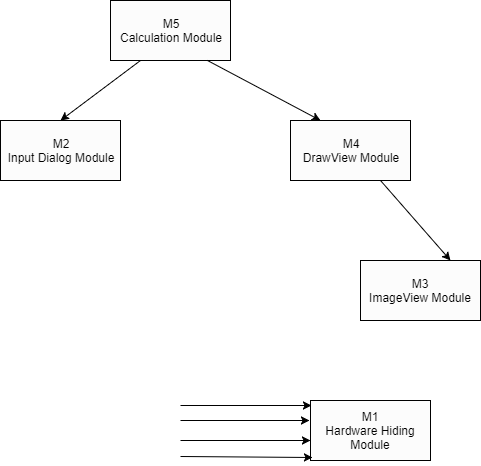
\includegraphics[width=0.7\textwidth]{UsesHierarchy.png}
\caption{Use hierarchy among modules}
\label{FigUH}
\end{figure}


\end{document}